\documentclass[xcolor=dvipsnames,beamer]{beamer} %handout,notes=show

\usepackage{textcomp}
\usepackage[utf8]{inputenc}
% \usepackage{default}
\usepackage{graphicx}
%  \usepackage[pdftex]{hyperref}
\usepackage{url}
\usepackage{amsmath}

% frames have to be fragile
\newif\ifnotes
% \notestrue

%\notestrue


\ifnotes
%\setbeamertemplate{note page}[plain]
\setbeamertemplate{note page}[compress]
\setbeamerfont{note page}{size=\large}
\setbeameroption{show only notes}
%\setbeameroption{show notes}
\usepackage{pgfpages}
\pgfpagesuselayout{2 on 1}[a4paper,border shrink=5mm]%
\else
%\setbeameroption{hide notes}
\fi
%\notesfalse



% nastaveni TypeWriter
%\usepackage{courier}
%\usepackage{lmodern}
%\renewcommand*\ttdefault{txtt}
\DeclareFontShape{OT1}{cmtt}{bx}{n}{<5><6><7><8><9><10><10.95><12><14.4><17.28><20.74><24.88>cmttb10}{}


% \usepackage{verbatim}
\usepackage[absolute,overlay]{textpos}

\usepackage{listings}
% \usepackage{courier}
\definecolor{grey}{RGB}{70,70,70}
\definecolor{green}{RGB}{0,255,0}
\definecolor{red}{RGB}{202,53,53}
\definecolor{lightGrey}{RGB}{250,250,250}
\definecolor{darkGrey}{RGB}{50,50,50}


\usepackage{color}
\definecolor{lightgray}{rgb}{.9,.9,.9}
\definecolor{darkgray}{rgb}{.4,.4,.4}
\definecolor{purple}{rgb}{0.65, 0.12, 0.82}


% \usetheme{Warsaw}
\usetheme{Madrid}
% \usetheme{Szeged}
% \useoutertheme{infolines}
\usecolortheme[named=MidnightBlue]{structure}
% \usecolortheme[named=PineGreen]{structure}
% \setbeamertemplate{navigation symbols}{}




\title[crowdsourcing ET calibration]
{GRASS GIS crowdsourcing of the local calibration of ETa models to improve on public domain Global ET products}
%\subtitle{SVO\v{C}}
%\pdforstring{}{}
\author[Yann Chemin]
{Yann Chemin}

\institute[IWMI]
{International Water Management Institute\\
\vspace{20pt}
% 
\includegraphics[width=1cm]{iwmi}
}
\date{April 16, 2013}


%\AtBeginSection[]{\begin{frame}\frametitle{Obsah}%
%\tableofcontents[currentsection ]\end{frame}}
%\AtBeginSubsection[]
%{
%  \begin{frame}<beamer>
%  \frametitle{Obsah}
%  \tableofcontents[currentsection,currentsubsection]
%  \end{frame}
%}

\setbeamercovered{transparent}

\hypersetup{%
	pdfauthor={Yann Chemin},%
	pdfsubject={Presentation},%
    pdfkeywords={GRASS, GIS, Evapotranspiration, crowdsourcing}
}

\usepackage{listings}
\lstdefinestyle{C++}{%
  % language
  language=C++, % [ANSI]C++, GNU, ISO, Visual
  basicstyle=\ttfamily\small,
  commentstyle=\itshape,
  keywordstyle=\bfseries, % needs another \ttdefault
  showstringspaces=false,
  stringstyle=,
  identifierstyle=,
  % working with latex
  escapeinside={//lst}{\^^M}  
}

\lstset{%
%  frame=trBL,
%  backgroundcolor=\color{},
  linewidth=\textwidth,
  % working with latex
  gobble=2,
  % float
  nolol=false,
  numberbychapter=true,
  captionpos=t,% tb
  % breaking lines
  breaklines=true,
  breakatwhitespace=true,
  breakindent=10em,
  breakautoindent=true,
  prebreak={},
  postbreak={},
  %document default style
    basicstyle=\ttfamily
}


%\lstlistlistingname % The header name for the list of listings.
%\lstlistingname % The caption label for listings.

\lstnewenvironment{cmdline}[1][]
{\lstset{
  style=C++,
  #1}}
{}

\lstnewenvironment{scpp}[1][]
{\lstset{
  style=C++,
  #1}}
{}

\lstnewenvironment{ncpp}[1][]
{\lstset{
  style=C++,
  numbers=left, 
  numberstyle=\scriptsize, 
  stepnumber=1,
  numbersep=5pt,
  #1}}
{}

\lstnewenvironment{fcpp}[1][]
{\lstset{
  style=C++,
  float,
   % line numbers
  numbers=left, 
  numberstyle=\scriptsize, 
  stepnumber=1,
  numbersep=5pt,
  #1}}
{}


\lstnewenvironment{lcpp}[1][]
{\lstset{%
style=C++,
numbers=left, 
numberstyle=\scriptsize, 
stepnumber=1,
numbersep=5pt,
xleftmargin=12pt,
breakautoindent=false,
breaklines=false,%
#1}}{}

\lstnewenvironment{smallcpp}[1][]
{\lstset{%
style=C++,
numbers=left, 
numberstyle=\tiny, 
stepnumber=1,
numbersep=5pt,
xleftmargin=12pt,
breakautoindent=false,
breaklines=false,%
basicstyle=\ttfamily\scriptsize,
#1}}{}


\lstnewenvironment{pscpp}[1][]
{\lstset{%
style=C++,
xleftmargin=12pt,
breakautoindent=false,
breaklines=false,
#1}}{}


%\lstset{index={square},index={[2]root}}


\newcommand{\overovaciref}[1]{{\scriptsize(\ref{#1})}}


\usepackage{tipa}
\newcommand{\pron}[2]{#1 [#2]}

%%%%%%%%%%%%%%%%%%%%%%%%%%%%%%%%%%%%%%%%%%%%%%%%%%%%%%%%%%%%%%%%%%%%
%%%%%%%%%%%%%%%%%%%%%%%%%%%%%%%%%%%%%%%%%%%%%%%%%%%%%%%%%%%%%%%%%%%%
%%%%%%%%%%%%%%%%%%%%%%%%%%%%%%%%%%%%%%%%%%%%%%%%%%%%%%%%%%%%%%%%%%%%
%%%%%%%%%%%%%%%%%%%%%%%%%%%%%%%%%%%%%%%%%%%%%%%%%%%%%%%%%%%%%%%%%%%%
\begin{document}
%%%%%%%%%%%%%%%%%%%%%%%%%%%%%%%%%%%%%%%%%%%%%%%%%%%%%%%%%%%%%%%%%%%%
\frame{
\titlepage
}
%%%%%%%%%%%%%%%%%%%%%%%%%%%%%%%%%%%%%%%%%%%%%%%%%%%%%%%%%%%%%%%%%%%%%
\begin{frame}{Contents}
\tableofcontents
\end{frame}
%%%%%%%%%%%%%%%%%%%%%%%%%%%%%%%%%%%%%%%%%%%%%%%%%%%%%%%%%%%%%%%%%%%%

\section{Introduction}
%%%%%%%%%%%%%%%%%%%%%%%%%%%%%%%%%%%%%%%%%%%%%%%%%%%%%%%%%%%%%%%%%%%%
\begin{frame}[fragile]{Overview}

Evapotranspiration is the largest transiting quantity in the daily 
hydrological cycle along with rain. It is used by scientists and
managers in:
\newline\linebreak

\begin{itemize}
 \item Irrigation systems performance
 \item Crop water productivity
 \item Water accounting
 \item Wetlands-agriculture interface
 \item Basin water uses quantification
 \item Climate change on water cycle \& users
\end{itemize}


\end{frame}

\section{Evapotranspiration Modeling}
\subsection{Overview}
%%%%%%%%%%%%%%%%%%%%%%%%%%%%%%%%%%%%%%%%%%%%%%%%%%%%%%%%%%%%%%%%%%%%
\begin{frame}[fragile]{Overview}

There are several types of evapotranspiration modeling methods:\\

\begin{itemize}
 \item Reference ET: Hargreaves, Penman-Monteith
 \item Potential ET: Priestley-Taylor, astronomical
 \item Actual ET: Thermodynamic/energy balance (mostly)
\end{itemize}

\end{frame}

\subsection{ETo \& ETpot}
%%%%%%%%%%%%%%%%%%%%%%%%%%%%%%%%%%%%%%%%%%%%%%%%%%%%%%%%%%%%%%%%%%%%
\begin{frame}[fragile]{Reference \& potential ET}

\begin{block}{Trunk (G7)}
\begin{itemize}
 \item i.evapo.mh: ETo Hargreaves, Modified H., H.-Samani 
 \item i.evapo.pm: ETo Penman-Monteith (PM, 1972)
 \item i.evapo.pt: ETpot Priestley-Taylor (PT, 1970s)
 \item i.evapo.potrad: ETpot astronomical (WB, 1995)
\end{itemize}
\end{block}

\begin{block}{Add-ons (G7)}
\begin{itemize}
 \item i.evapo.senay: ET \textit{regional} (Senay, 2007)
 \item i.evapo.zk: ET \textit{biome} (ZK, 2010)
\end{itemize}
\end{block}
\end{frame}

\subsection{ETa definition}
%%%%%%%%%%%%%%%%%%%%%%%%%%%%%%%%%%%%%%%%%%%%%%%%%%%%%%%%%%%%%%%%%%%%
\begin{frame}[fragile]{Actual ET}

Actual ET: thermodynamic heat flux modeling\\

\begin{equation}\label{eq1}
\Lambda = \frac {Rn - G - H} {Rn - G}
\end{equation}

\begin{equation}\label{eq2}
ET_a = \Lambda \, ET_{potential}
\end{equation}

\begin{block}{i.eb.* modules (G7 main) using thermodynamic heat flux modeling}
\begin{itemize}
 \item i.eb.netrad: Net radiation (Rn in \ref{eq1}) 
 \item i.eb.h\_*: Sensible heat flux (H in \ref{eq1})
 \item i.eb.evapfr: Evaporative fraction ($\Lambda$ in \ref{eq2})
 \item i.eb.eta: Evapotranspiration (ETa in \ref{eq2})
\end{itemize}
\end{block}
\end{frame}

\subsection{ETa examples 1}
%%%%%%%%%%%%%%%%%%%%%%%%%%%%%%%%%%%%%%%%%%%%%%%%%%%%%%%%%%%%%%%%%%%%
\begin{frame}[fragile]{Evapotranspiration @ country level}

Actual evapotranspiration\\ 
for water resources monitoring \& management.\\

\begin{center}
 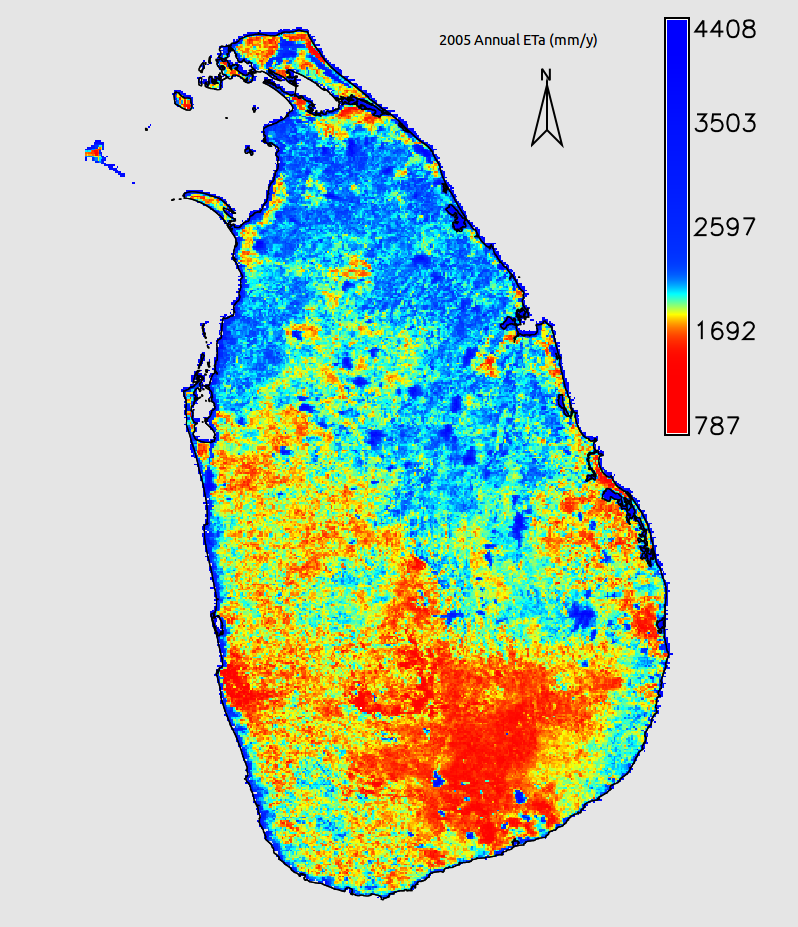
\includegraphics[width=5cm]{slet2005}
 \hspace{10mm}
 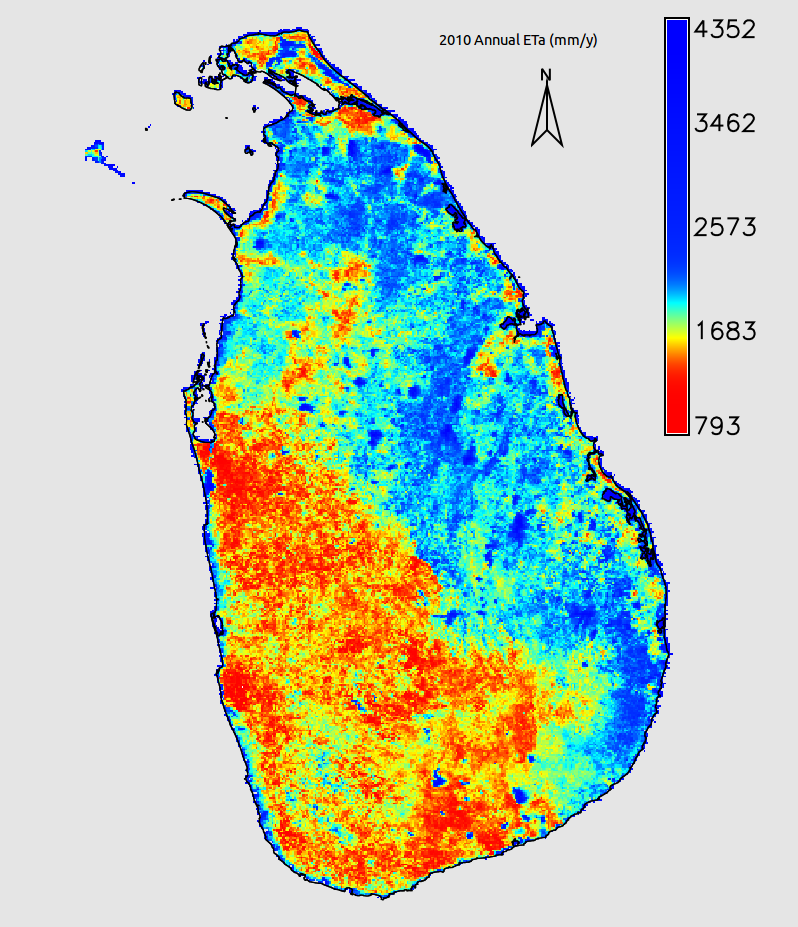
\includegraphics[width=5cm]{slet2010}
\end{center}

\end{frame}

\subsection{ETa examples 2}
%%%%%%%%%%%%%%%%%%%%%%%%%%%%%%%%%%%%%%%%%%%%%%%%%%%%%%%%%%%%%%%%%%%%
\begin{frame}[fragile]{Equity of water use in irrigation systems}

Irrigation water monitoring \& management
\begin{itemize}
 \item Map: Uniform colour is equity of water distribution
 \item Graph: irrigation system equity in time (daily, 12 years)
\end{itemize}

\begin{columns}[l]
\column{0.2\textwidth}
\begin{center}
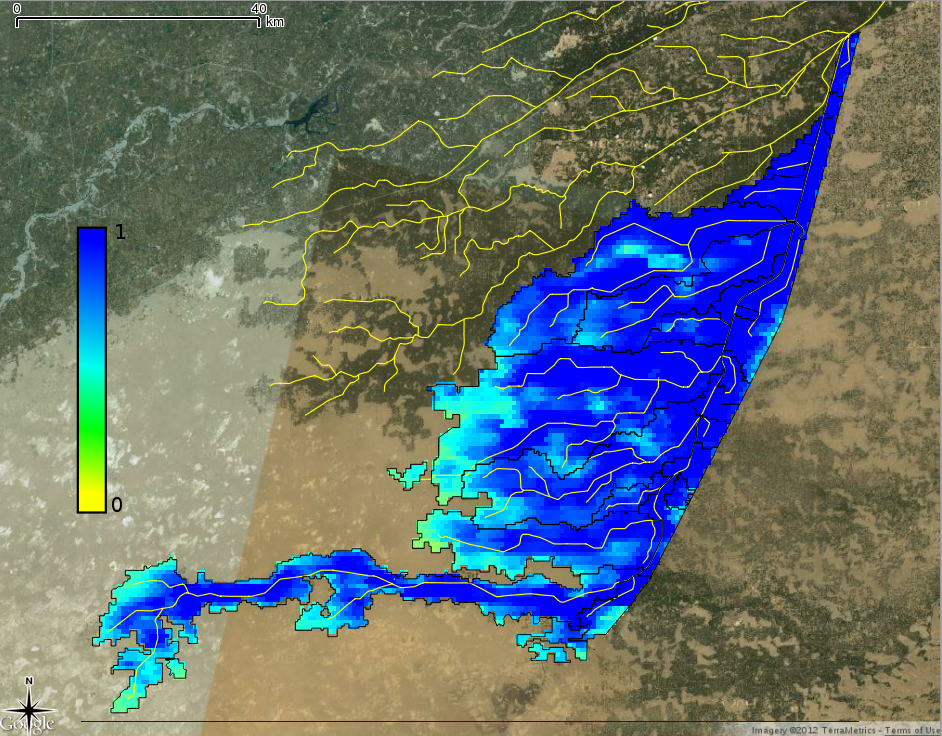
\includegraphics[width=4cm]{fess2012ef}
\end{center}

\column{0.8\textwidth}
\begin{flushright}
  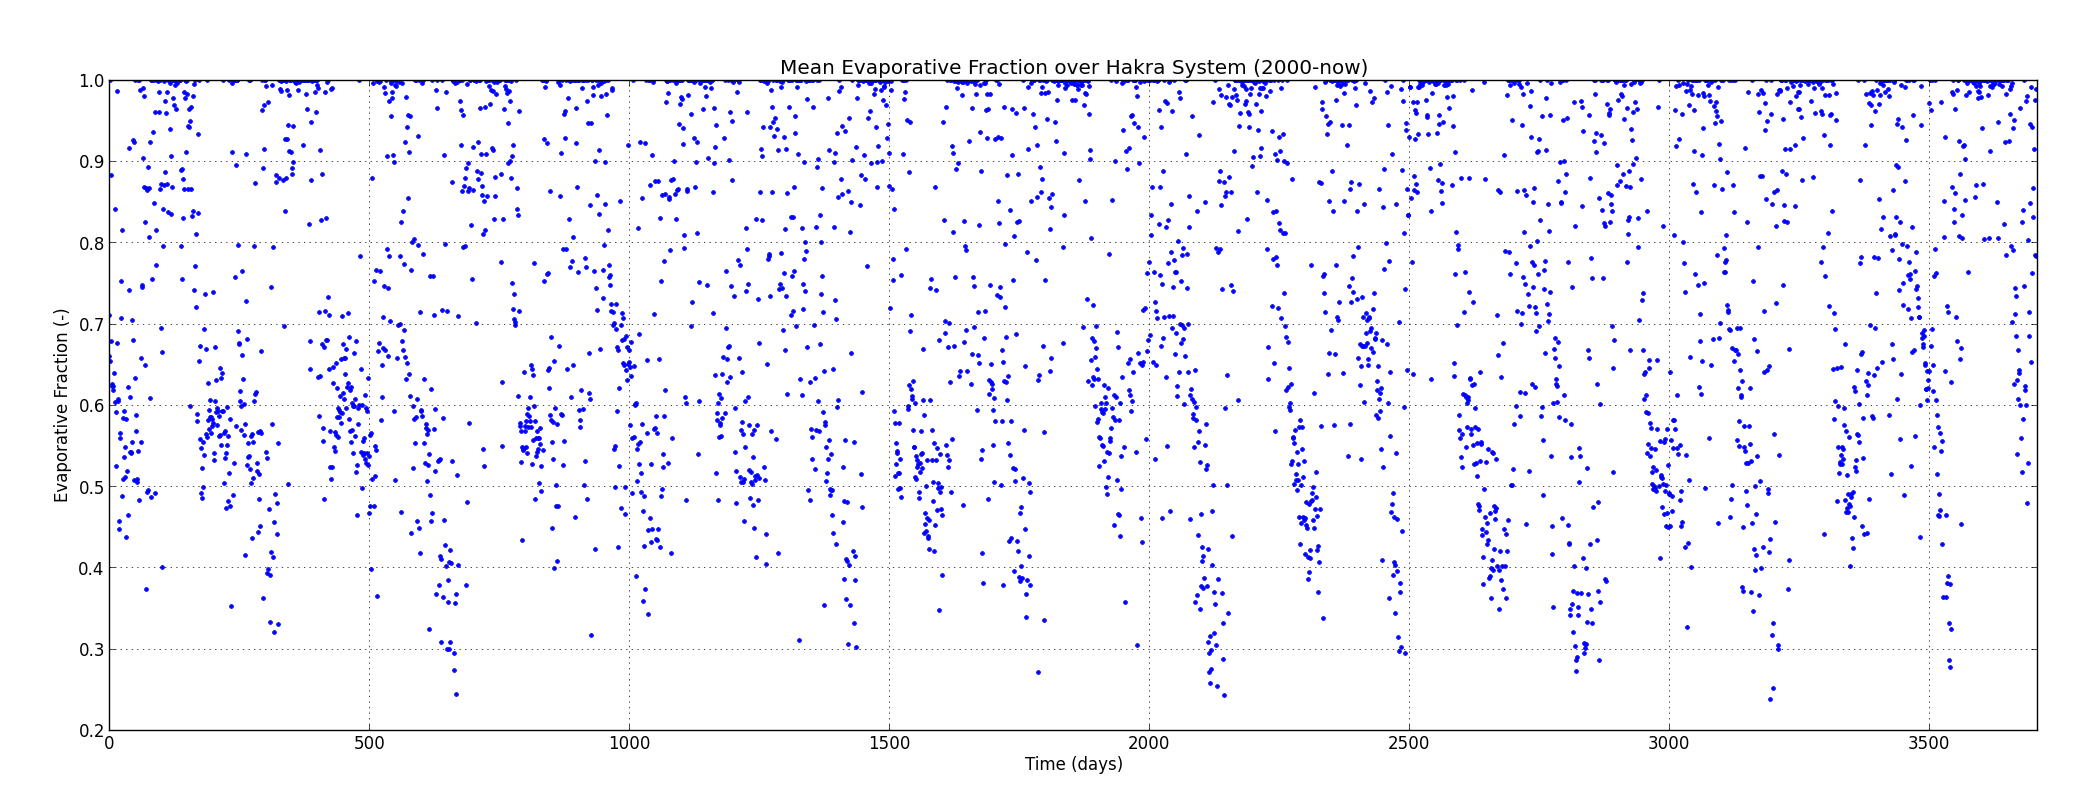
\includegraphics[width=8cm]{fess2012meaneftemporal}
\end{flushright}
\end{columns}

\end{frame}

\subsection{ETa examples 3}
%%%%%%%%%%%%%%%%%%%%%%%%%%%%%%%%%%%%%%%%%%%%%%%%%%%%%%%%%%%%%%%%%%%%
\begin{frame}[fragile]{Crop water consumption in irrigation systems}

Actual evapotranspiration (mm/d)\\ 
for agricultural water performance management.\\

\begin{center}
 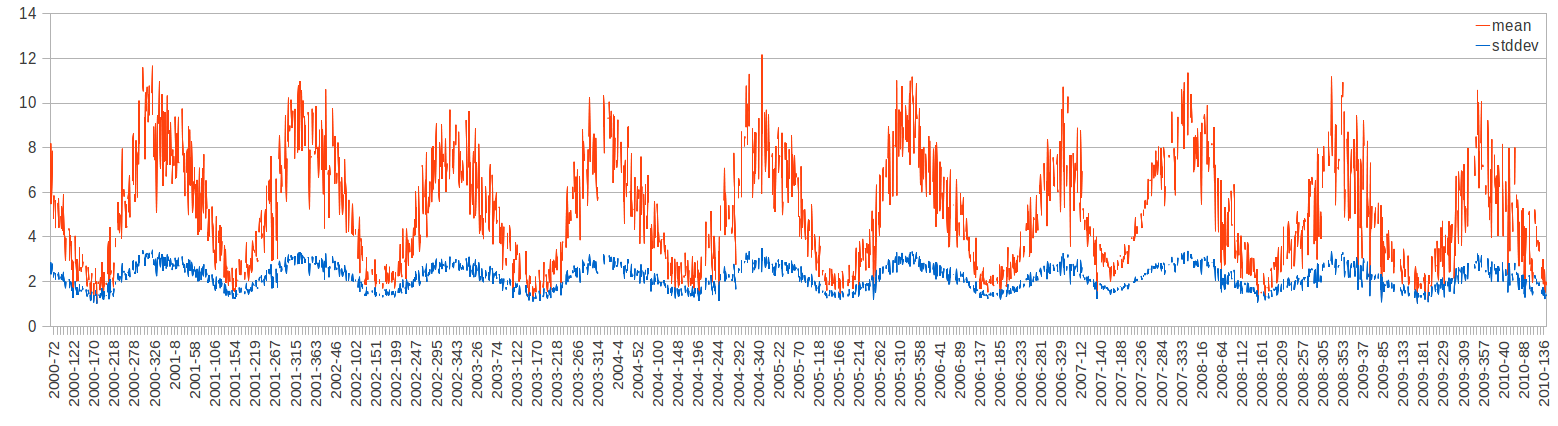
\includegraphics[width=9.5cm]{ciameanet}\\
 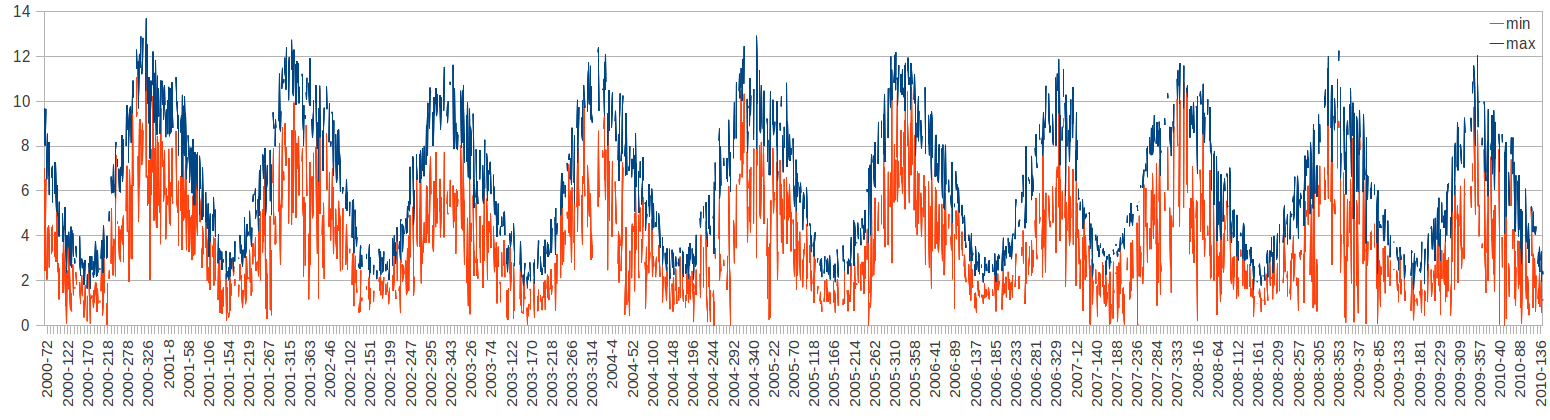
\includegraphics[width=9.5cm]{ciaminmaxet}
\end{center}

\end{frame}

\subsection{Chain processing}
%%%%%%%%%%%%%%%%%%%%%%%%%%%%%%%%%%%%%%%%%%%%%%%%%%%%%%%%%%%%%%%%%%%%
\begin{frame}[fragile]{Chain processing}

Chain processing has a fundamental impact on remote sensing work:\\

\begin{itemize}
 \item Standardization limits bugs
 \item Less prone to human error
 \item Simpler parameterization access
 \item Permits to apply any number of modules to all target images
 \item Ensures maximum quality of generated images
\end{itemize}


\begin{block}{Concept}
\begin{itemize}
 \item META Module, a module using modules
 \item Prototype, shell script, then grass.script
 \item Actually moving to pygrass (Genoa CS2013)
\end{itemize}
\end{block}

\end{frame}
%%%%%%%%%%%%%%%%%%%%%%%%%%%%%%%%%%%%%%%%%%%%%%%%%%%%%%%%%%%%%%%%%%%%
\begin{frame}[fragile]{Chain processing}

The development of pyGRASS is maturing,\\
META Modules arise from vertical integration.

\begin{center}
 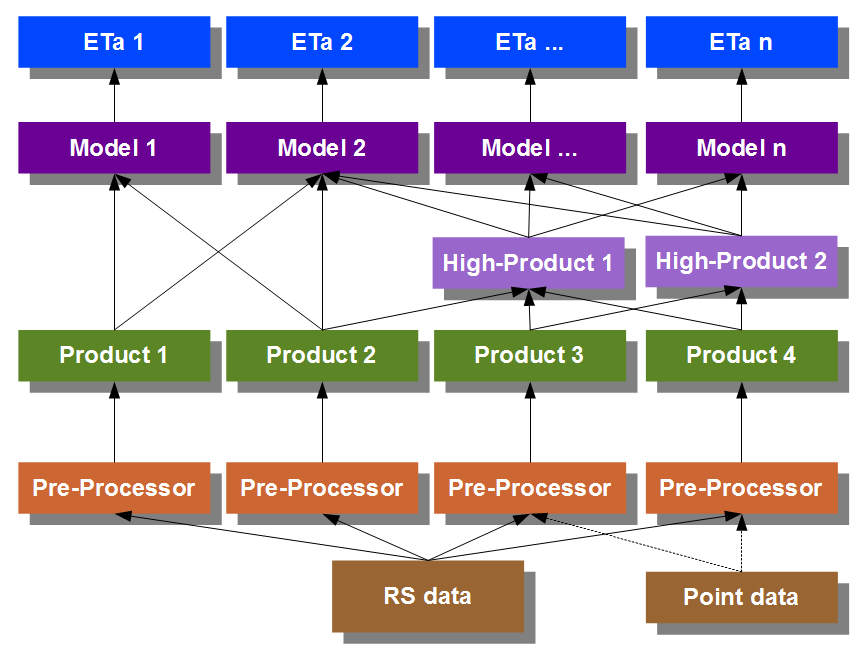
\includegraphics[width=7.5cm]{chain0}
\end{center}

\end{frame}

\subsection{MOD 16}
%%%%%%%%%%%%%%%%%%%%%%%%%%%%%%%%%%%%%%%%%%%%%%%%%%%%%%%%%%%%%%%%%%%%
\begin{frame}[fragile]{MOD16 MODIS product}

Global monthly (MOD16A2) and yearly (MOD16A3) dataset
\begin{center}
 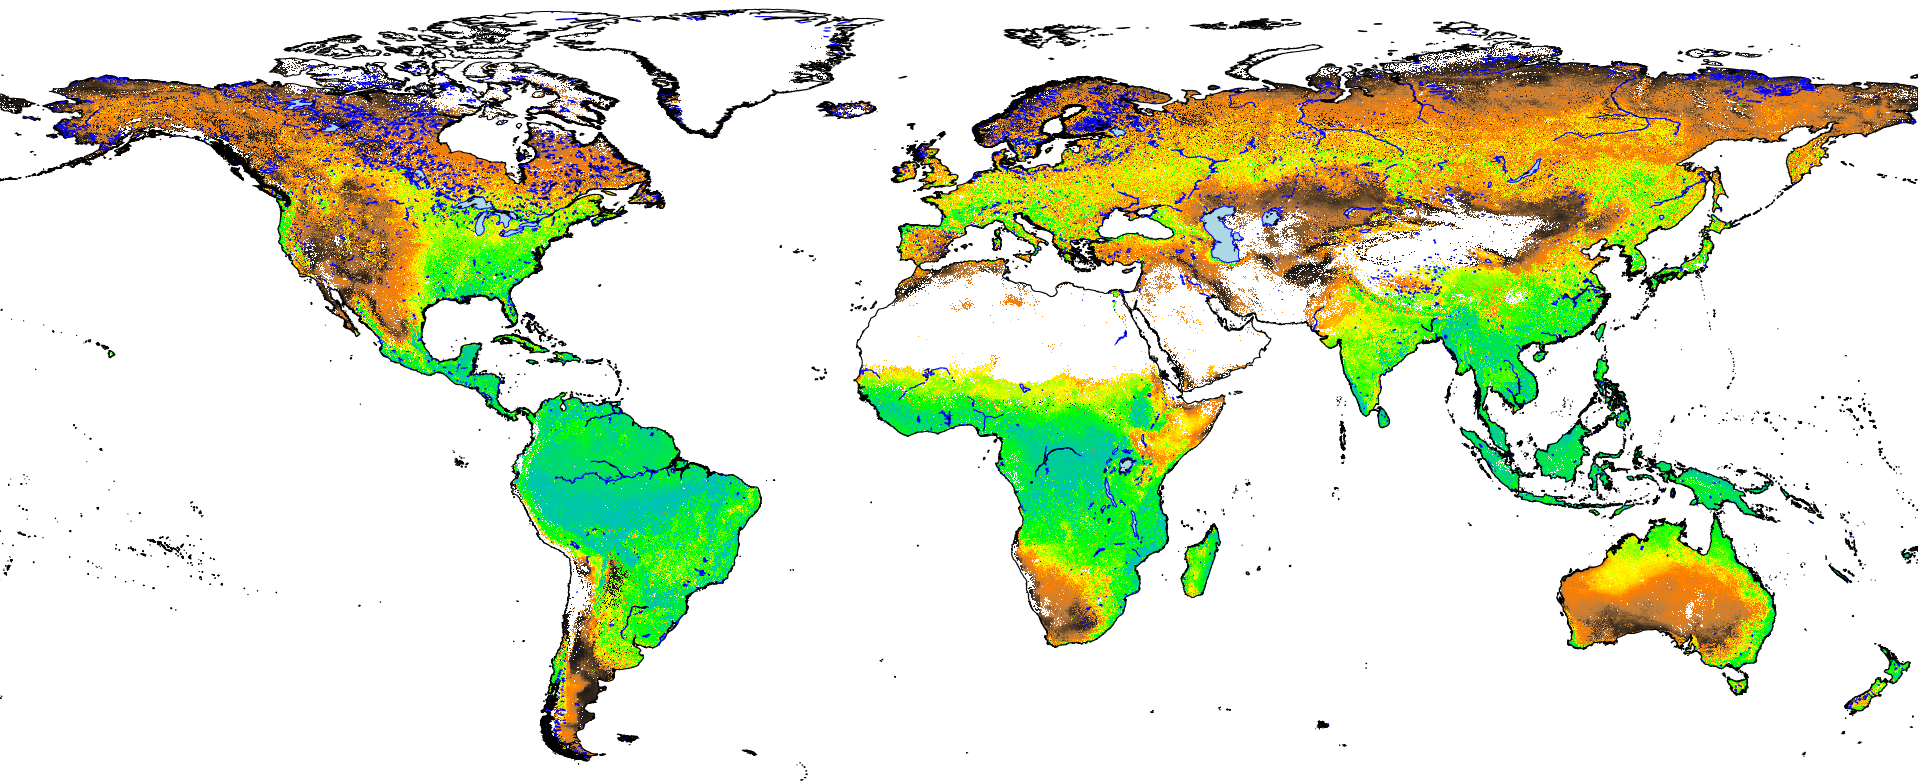
\includegraphics[width=10.5cm]{MOD16_2000.png}
\end{center}
8km parameterization, validated on Fluxnet data.\\
Not validated daily.
\end{frame}


\section{Crowdsourcing}
\subsection{Rationale}
%%%%%%%%%%%%%%%%%%%%%%%%%%%%%%%%%%%%%%%%%%%%%%%%%%%%%%%%%%%%%%%%%%%%
\begin{frame}[fragile]{Rationale for crowdsourcing}

\begin{columns}[l]
\column{0.7\textwidth}
Local parameterization of ET models is necessary\newline\linebreak

\begin{block}{because the end-user is:}
\begin{itemize}
 \item in a better position for QC in/out
 \item interested in both upstream/downstream
\end{itemize}
\end{block}

\begin{block}{but the constraints are:}
\begin{itemize}
 \item using ET models
 \item using GIS, FOSSGIS
\end{itemize}
\end{block}
\column{0.3\textwidth}
\begin{center}
 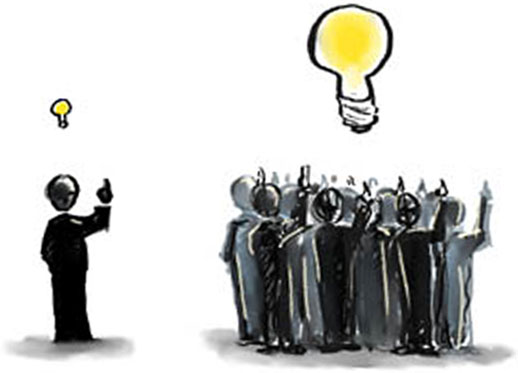
\includegraphics[width=3.5cm]{crowdsourcing}
\end{center}
\end{columns}

\end{frame}

\subsection{Year 1}
%%%%%%%%%%%%%%%%%%%%%%%%%%%%%%%%%%%%%%%%%%%%%%%%%%%%%%%%%%%%%%%%%%%%
\begin{frame}[fragile]{set up for year 1: Kick the geek}

Scientists on all continents
\begin{itemize}
 \item Background in RS/ET/FOSS (pick any to all)
 \item Interested to publish their calibration of ET models
 \item Willing to be trained on GRASS GIS v7
\end{itemize}


\begin{block}{Year 1 Goals}
\begin{itemize}
 \item Training a core of interested scientists
 \item GRASS GIS modules for ET modeling taken over by users
\end{itemize}
\end{block}

\end{frame}

\subsection{Year 2}
%%%%%%%%%%%%%%%%%%%%%%%%%%%%%%%%%%%%%%%%%%%%%%%%%%%%%%%%%%%%%%%%%%%%
\begin{frame}[fragile]{set up for year 2: Bring the bee}

Any interested person on all continents
\begin{itemize}
 \item Background in science
 \item Interested to learn that knowledge
 \item Willing to be trained on GRASS GIS
 \item Interested in simple GRASS GIS raster programming
\end{itemize}

\begin{block}{Year 2 Goals}
\begin{itemize}
 \item Year 1 articles in press, local calibration in svn
 \item HPC FOSS source code online
 \item GRASS GIS ET modules used by Year 2 community
\end{itemize}
\end{block}

\end{frame}

\subsection{Year 3}
%%%%%%%%%%%%%%%%%%%%%%%%%%%%%%%%%%%%%%%%%%%%%%%%%%%%%%%%%%%%%%%%%%%%
\begin{frame}[fragile]{set up for year 3: Ubergeek upgrade}

Any intensely interested person on all continents
\begin{itemize}
 \item Background in C programming, ET models
 \item Interested to process all MODIS archives
 \item Willing to learn and contribute distributed modeling
\end{itemize}


\begin{block}{Year 3 Goals}
\begin{itemize}
 \item Year 1/2 articles in press
 \item Local calibration in svn
 \item HPC FOSS source code taken over by community
\end{itemize}
\end{block}

\end{frame}

\section{Conclusions}
%%%%%%%%%%%%%%%%%%%%%%%%%%%%%%%%%%%%%%%%%%%%%%%%%%%%%%%%%%%%%%%%%%%%
\begin{frame}[fragile]{Conclusions}

One for all
\begin{itemize}
 \item Crowdsourcing of science should be possible
 \item But needs supporting efforts in terms of training
 \item Realizing this makes the science uptake more robust
\end{itemize}

\begin{block}{All for all}
\begin{itemize}
 \item Returning local parameterization from local to svn
 \item Permits local QC improvement of global ET data generation
 \item Anybody can model ET anywhere/anywhen they want
\end{itemize}
\end{block}

\end{frame}

%%%%%%%%%%%%%%%%%%%%%%%%%%%%%%%%%%%%%%%%%%%%%%%%%%%%%%%%%%%%%%%%%%%%
\begin{frame}[fragile]{Thank You}

\begin{center}
 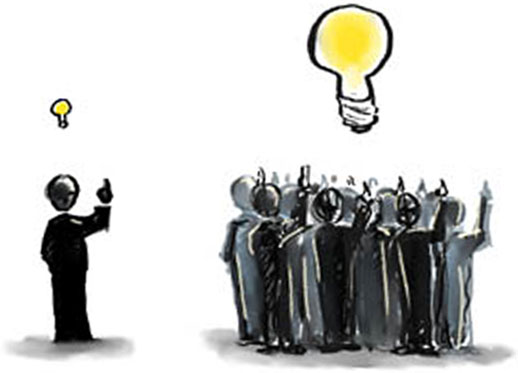
\includegraphics[width=5cm]{crowdsourcing}
\end{center}

\end{frame}

\end{document}
